\documentclass[11pt]{article}
\usepackage{../mymacros}

\setlength{\parindent}{0em}
\setlength{\parskip}{1em}

\begin{document}

% Set header and footer

\pagestyle{fancy}
\fancyhf{}
\rhead{PHYS 472}
\lhead{Assignment 2}
\cfoot{\thepage}

\begin{lstlisting}
    Plot[
        {2 \[Xi]^2 Exp[-2 \[Xi]^2], 4 \[Xi]^2 Exp[-2 \[Xi]^2], 0}, {\[Xi], -2, 2},
        PlotLegends -> {"distinguishable", "bosons", "fermions"}]
\end{lstlisting}

\begin{figure}[h!] % the [h!] argument attempts to place the figure here in the document
    \centering
    \resizebox{0.8\textwidth}{!}{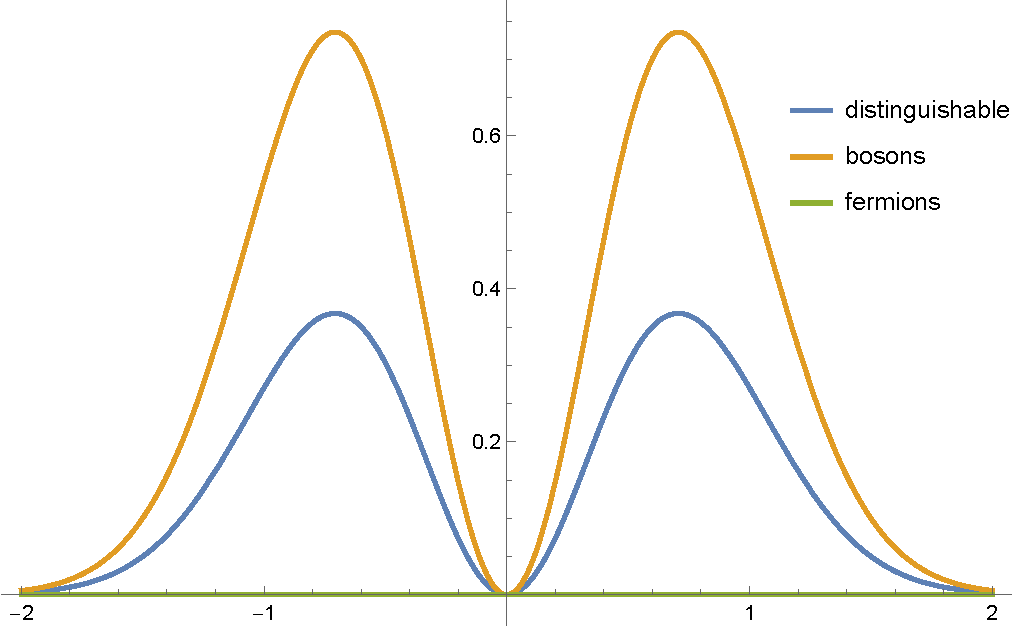
\includegraphics{atSamePosition.pdf}} % resizes the figure to 80% of the text width while maintaining the aspect ratio
    \caption{placeholder}
    \label{fig:fig1}
\end{figure}

\begin{lstlisting}
    plot1 = Plot3D[
        4 xi2^2 Exp[-xi1^2/2 - xi2^2/2], {xi1, -3, 3}, {xi2, -3, 3}, 
        AxesLabel -> {Subscript[\[Xi], 1], Subscript[\[Xi], 2], 
        Superscript[Abs[Subscript[\[Psi], Row[{"(", Subscript[\[Xi], 1], ", ", Subscript[\[Xi], 2], ")"}]]], 2]}, PlotStyle -> Opacity[0.5], Mesh -> None, PlotRange -> All];

    plot2 = Plot3D[
        4 xi2^2 Exp[-xi1^2/2 - xi2^2/2] (xi1 + xi2)^2, {xi1, -3, 
        3}, {xi2, -3, 3}, PlotStyle -> {Opacity[0.5], Red}, Mesh -> None, PlotRange -> All];

    plot3 = Plot3D[
        4 xi2^2 Exp[-xi1^2/2 - xi2^2/2] (xi1 - xi2)^2, {xi1, -3, 
        3}, {xi2, -3, 3}, PlotStyle -> {Opacity[0.5], Blue}, Mesh -> None, PlotRange -> All];

    atDifferentPosition = Show[
        Legended[plot1, Placed[Style["distinguishable", FontColor -> Orange], {0.15, 0.8}]], 
        Legended[plot2, Placed[Style["bosons", FontColor -> Red], {0.15, 0.8}]], 
        Legended[plot3, Placed[Style["fermions", FontColor -> Blue], {0.15, 0.8}]],ViewPoint -> {2.7, -3.5, 2.5}]
\end{lstlisting}

\begin{figure}[h!] % the [h!] argument attempts to place the figure here in the document
    \centering
    \resizebox{1\textwidth}{!}{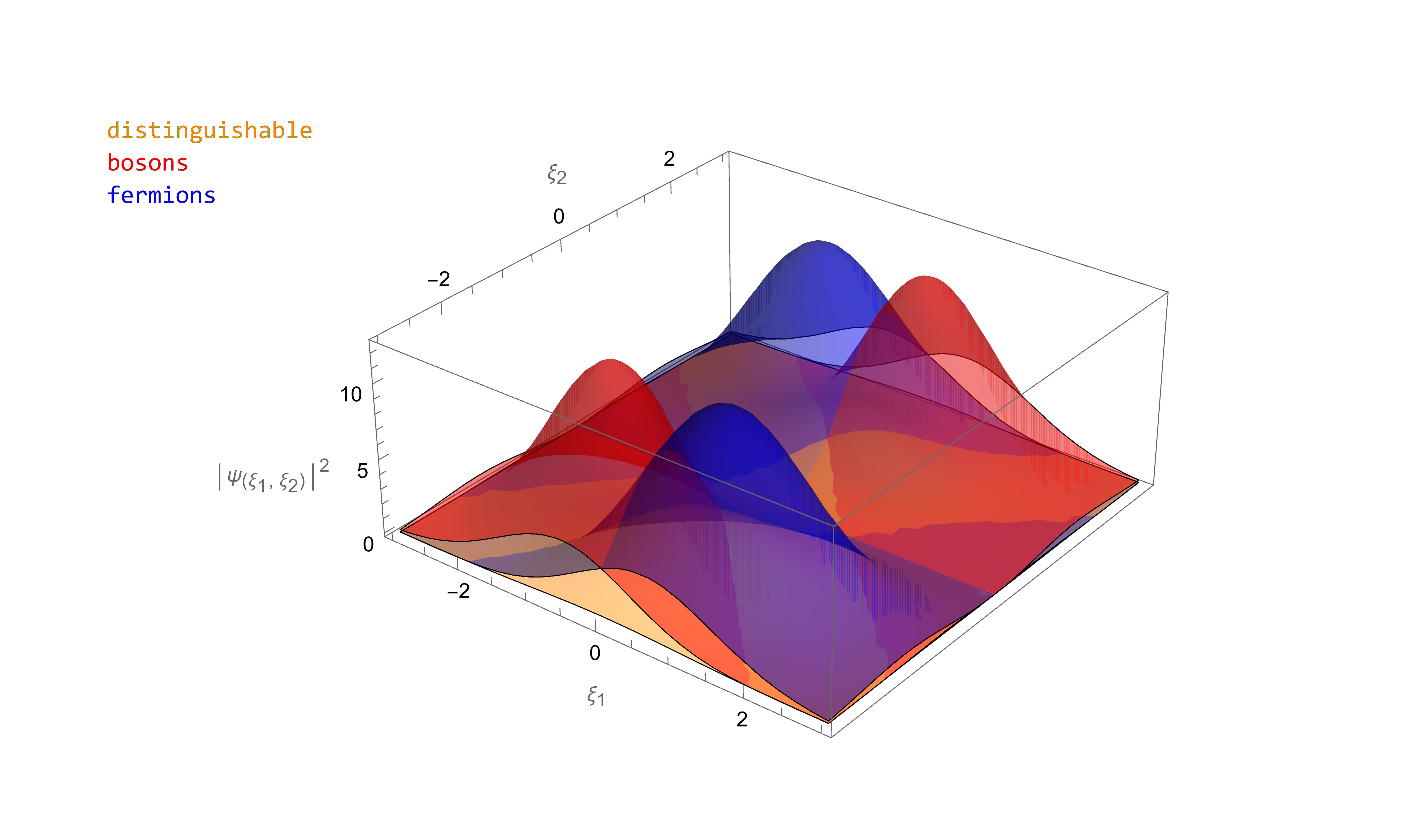
\includegraphics{atDifferentPosition.pdf}} % resizes the figure to 80% of the text width while maintaining the aspect ratio
    \caption{placeholder}
    \label{fig:fig2}
\end{figure}
    



\end{document}